\chapter{Экспериментальное исследование и анализ результатов}
\label{ch4}

\vspace{0.5cm}

В данной главе представлены результаты экспериментального исследования модифицированного аукционного алгоритма, описанного в главе \ref{ch2}, в сравнении с классическим венгерским алгоритмом. Рассматриваются модельные задачи, имитирующие распределенные системы роботов с различной топологией сети связи, определяемой радиусом видимости \( r_v \). Описываются метрики оценки, включающие время выполнения, количество операций и относительную точность. Анализируется эффективность предложенного алгоритма, проверяются гипотезы, сформулированные в главе \ref{ch2}. Результаты визуализированы в виде графиков.

\section{Постановка эксперимента}

\subsection{Модельные задачи}

\vspace{0.3cm}

Для исследования эффективности модифицированного аукционного алгоритма были разработаны модельные задачи, имитирующие распределенные системы роботов. Параметры задач включали:

\begin{itemize}
    \item \textbf{Размер задачи}: Число роботов \( n \) и задач \( m \) варьировалось от 5 до 100, при этом \( n = m \) для сбалансированной задачи.
    \item \textbf{Радиус видимости}: Рассматривались значения \( r_v \in \{10, 20, 30\} \), а также диапазон от 5 до 100 для анализа влияния радиуса на точность.
    \item \textbf{Координаты}: Координаты роботов \( \{p_i = (x_i, y_i)\} \) и задач \( \{q_j = (x_j, y_j)\} \) генерировались случайным образом в диапазоне \( [1, 100] \) с использованием генератора псевдослучайных чисел.
    \item \textbf{Матрица выгод}: Выгода \( \alpha_{ij} \) определялась как:
    \[
    \alpha_{ij} = \frac{100}{d(p_i, q_j) + \delta},
    \]
    где \( d(p_i, q_j) \) --- евклидово расстояние, \( \delta \) --- константа для предотвращения деления на ноль.
    \item \textbf{Матрица видимости}: Матрица \( V = \{v_{ij}\} \) формировалась так, что \( v_{ij} = 1 \), если \( d(p_i, p_j) \leq r_v \), и \( v_{ij} = 0 \) в противном случае.
    \item \textbf{Параметр \( \varepsilon \)}: Для аукционного алгоритма исследовались значения \( \varepsilon \) от \( 10^{-5} \) до 10 с логарифмическим шагом.
\end{itemize}

Каждая задача генерировалась 100 раз для усреднения результатов, что обеспечивало статистическую надежность.

\subsection{Метрики оценки}

\vspace{0.3cm}

Для сравнения алгоритмов использовались следующие метрики:

\begin{itemize}
    \item \textbf{Время выполнения}: Измерялось в миллисекундах и усреднялось по 100 запускам для каждого набора параметров (\( n, r_v, \varepsilon \)).
    \item \textbf{Количество операций}: Определялось как число итераций алгоритмов для фиксированного радиуса \( r_v = 200 \).
    \item \textbf{Относительная точность}: Вычислялась как:
    \[
    \text{Точность} = \frac{A_{\text{auction}}}{A_{\text{hungarian}}} \cdot 100\%,
    \]
    где \( A_{\text{auction}} \) --- суммарная выгода аукционного алгоритма, \( A_{\text{hungarian}} \) --- суммарная выгода венгерского алгоритма (оптимальное решение).
\end{itemize}

\subsection{Методика проведения экспериментов}

Эксперименты проводились с использованием программной реализации на языке C++ с применением стандартных библиотек для обработки данных и построения графиков. Исследовались следующие аспекты:

\begin{enumerate}
    \item Сравнение времени выполнения аукционного и венгерского алгоритмов для различных размеров задачи и радиусов видимости.
    \item Оценка числа итераций для фиксированного радиуса \( r_v = 200 \).
    \item Анализ относительной точности аукционного алгоритма для фиксированных размеров задачи \( n \in \{10, 30, 50\} \) и различных радиусов.
    \item Исследование влияния параметра \( \varepsilon \) на время выполнения и точность при \( n = 80 \) и \( r_v \in \{10, 20, 30\} \).
    \item Оценка точности аукционного алгоритма на каждой итерации для \( n \in \{10, 30, 50, 100\} \) и \( r_v = 200 \).
\end{enumerate}

Результаты представлены в виде графиков, сохраненных в формате PNG.

\section{Результаты экспериментов}

\subsection{Время выполнения}

\vspace{0.3cm}

Эксперименты проводились для \( n = m \) от 5 до 100 и радиусов \( r_v \in \{10, 20, 30\} \). Результаты представлены на графике (см. рисунок \ref{fig:time_chart}).

\begin{figure}[h]
    \centering
    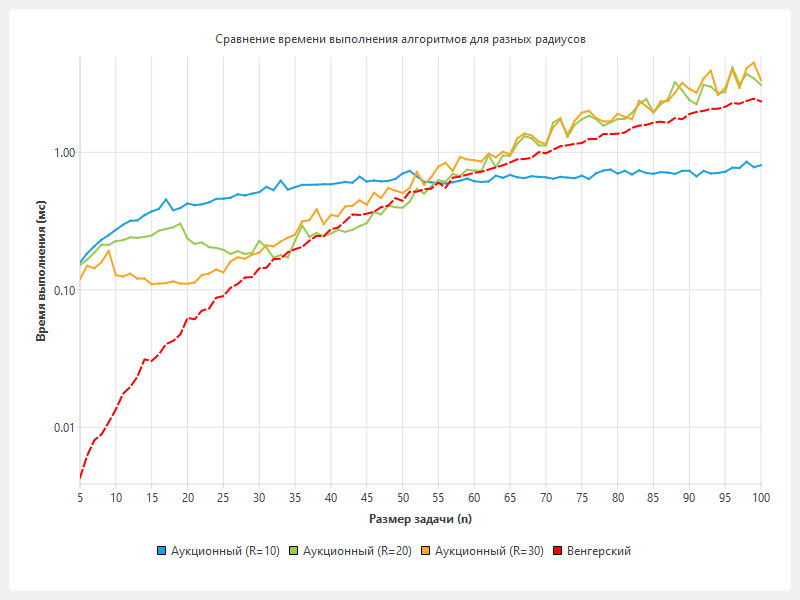
\includegraphics[width=0.8\textwidth]{my_folder/images/time_chart.png}
    \caption{Зависимость времени выполнения аукционного и венгерского алгоритмов от размера задачи для различных радиусов видимости.}
    \label{fig:time_chart}
\end{figure}

Основные наблюдения:
\begin{itemize}
    \item Время выполнения аукционного алгоритма возрастает с увеличением \( n \), но остается конкурентоспособным по сравнению с венгерским алгоритмом, особенно при больших \( r_v \).
    \item Увеличение радиуса видимости снижает время выполнения аукционного алгоритма за счет формирования более крупных связных компонент.
    \item Венгерский алгоритм демонстрирует более стабильное время выполнения, но его производительность ухудшается при больших \( n \) из-за сложности \( O(n^3) \).
\end{itemize}



\subsection{Относительная точность}
Точность аукционного алгоритма исследовалась для \( n \in \{10, 30, 50\} \) и \( r_v \) от 5 до 100 (см. рисунок \ref{fig:accuracy_chart}).

\begin{figure}[h]
    \centering
    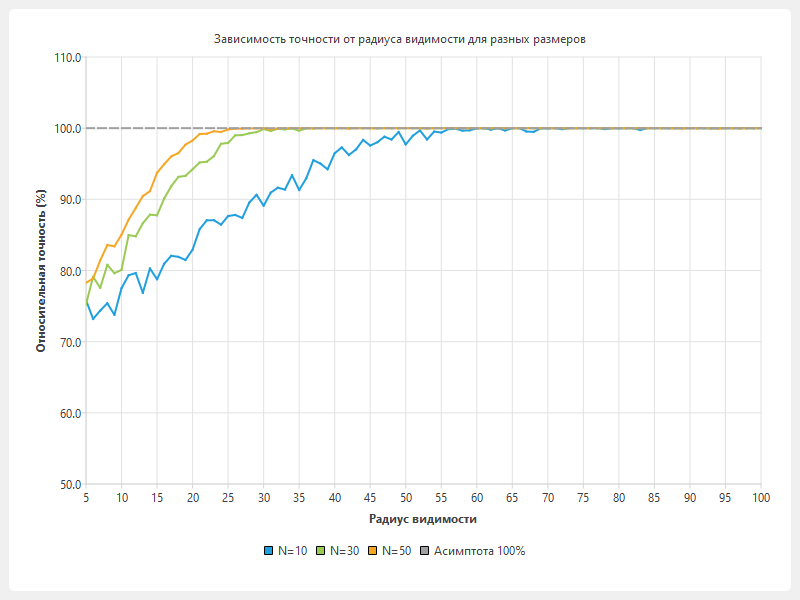
\includegraphics[width=0.8\textwidth]{my_folder/images/accuracy_chart.png}
    \caption{Зависимость относительной точности аукционного алгоритма от радиуса видимости для различных размеров задачи.}
    \label{fig:accuracy_chart}
\end{figure}

Выводы:
\begin{itemize}
    \item Точность возрастает с увеличением \( r_v \), достигая 95--100\% при \( r_v \geq 50 \) для малых \( n \).
    \item Для больших \( n \) точность возрастает быстрее из-за увеличения числа связных компонент.
\end{itemize}

\subsection{Влияние параметра \( \varepsilon \)}

\vspace{0.3cm}

Влияние \( \varepsilon \) на время и точность исследовалось для \( n = 80 \) и \( r_v \in \{10, 20, 30\} \) (см. рисунки \ref{fig:epsilon_time_chart} и \ref{fig:epsilon_accuracy_chart}).

\begin{figure}[h]
    \centering
    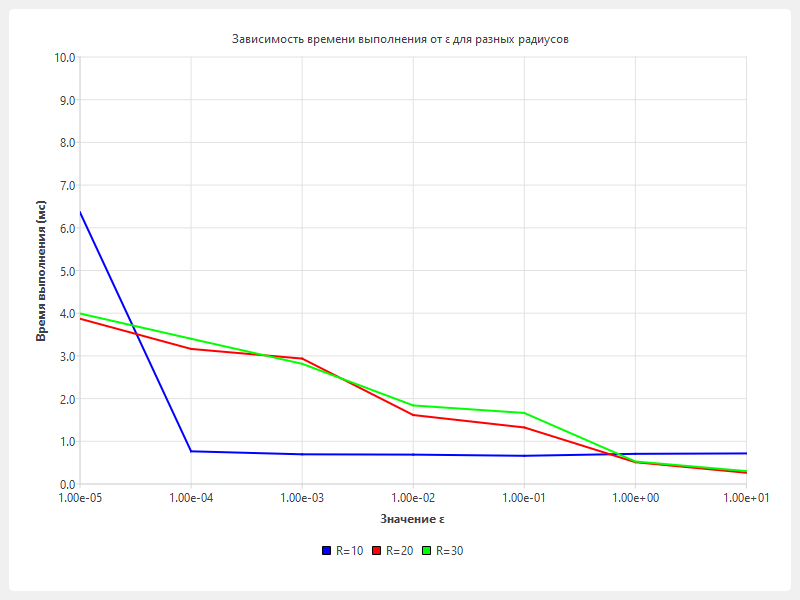
\includegraphics[width=0.8\textwidth]{my_folder/images/epsilon_time_chart.png}
    \caption{Зависимость времени выполнения аукционного алгоритма от \( \varepsilon \) для различных радиусов видимости.}
    \label{fig:epsilon_time_chart}
\end{figure}

\begin{figure}[h]
    \centering
    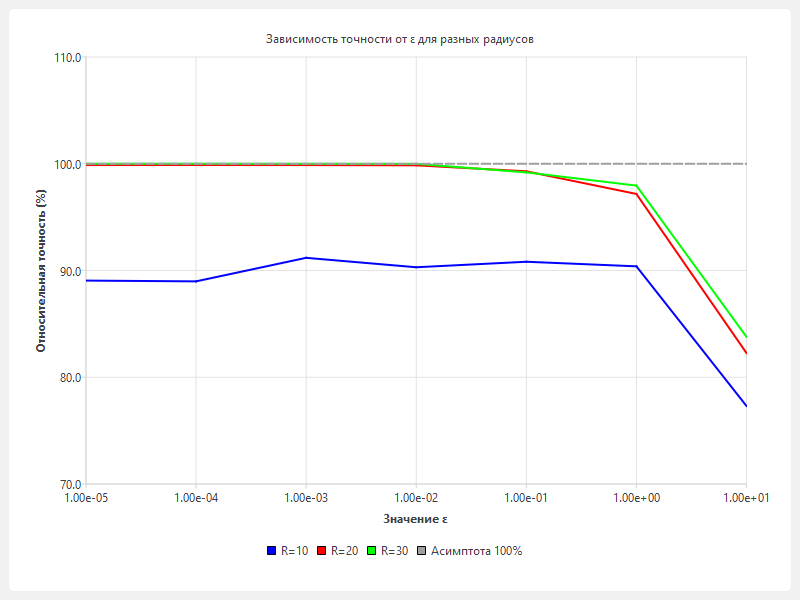
\includegraphics[width=0.8\textwidth]{my_folder/images/epsilon_accuracy_chart.png}
    \caption{Зависимость относительной точности аукционного алгоритма от \( \varepsilon \) для различных радиусов видимости.}
    \label{fig:epsilon_accuracy_chart}
\end{figure}

Наблюдения:
\begin{itemize}
    \item Время выполнения уменьшается с ростом \( \varepsilon \), так как требуется меньше итераций.
    \item Точность падает при больших \( \varepsilon \), но при \( \varepsilon \leq 10^{-2} \) превышает 90\%.
\end{itemize}

\subsection{Точность по итерациям}

\vspace{0.3cm}

Точность на каждой итерации исследовалась для \( n \in \{10, 30, 50, 100\} \) и \( r_v = 200 \) (см. рисунок \ref{fig:acc_per_iteration_chart}).

\begin{figure}[h]
    \centering
    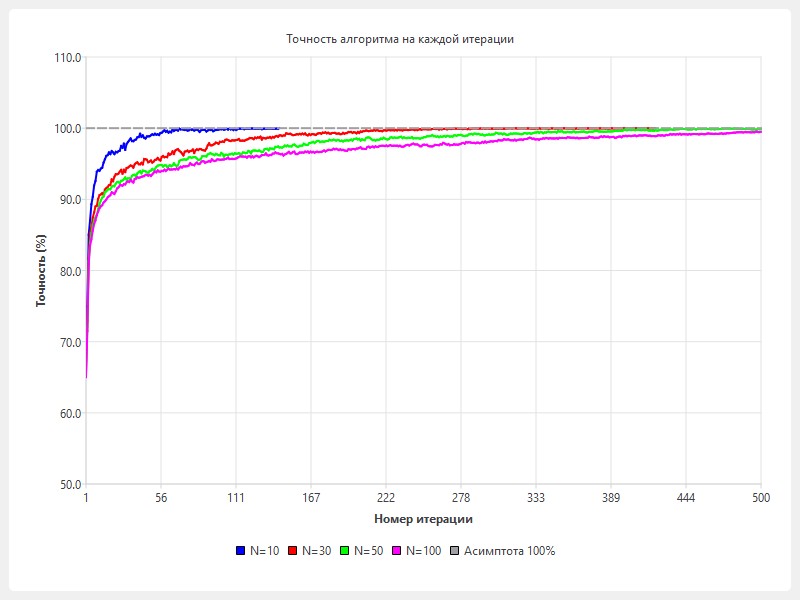
\includegraphics[width=0.8\textwidth]{my_folder/images/accuracy_per_iteration_chart.png}
    \caption{Зависимость относительной точности аукционного алгоритма от номера итерации для различных размеров задачи.}
    \label{fig:acc_per_iteration_chart}
\end{figure}

Наблюдения:
\begin{itemize}
    \item Точность быстро растет на первых итерациях, стабилизируясь на уровне 90--100\%.
    \item Для больших \( n \) требуется больше итераций из-за увеличения числа конфликтов.
\end{itemize}

\section{Анализ результатов}

Результаты подтверждают гипотезы, сформулированные в главе \ref{ch2}:

\begin{itemize}
    \item \textbf{Гипотеза 1}: Алгоритм завершается за конечное число шагов, а время выполнения пропорционально \( C / \varepsilon \), что подтверждается зависимостью времени от \( \varepsilon \) и \( r_v \).
    \item \textbf{Гипотеза 2}: Локальная оптимальность достигается в каждой связной компоненте при \( \varepsilon < 1/n \), но глобальная оптимальность ограничена числом компонент.
    \item \textbf{Гипотеза 3}: Высокая точность при небольших \( r_v \) указывает на потенциальную устойчивость в динамических сетях в условиях ограниченной связи.
\end{itemize}

Модифицированный аукционный алгоритм демонстрирует конкурентоспособное время выполнения и высокую точность (95--100\%) при подходящих параметрах.



\section{Выводы}

Модифицированный аукционный алгоритм показал эффективность в распределенных системах роботов, обеспечивая высокую точность и конкурентоспособное время выполнения. Параллельная обработка связных компонент снижает вычислительные затраты. Дальнейшие исследования могут быть направлены на тестирование алгоритма в динамических сетях и улучшение глобальной оптимальности.